\documentclass[letterpaper]{article}
\usepackage{natbib,alifexi}
\usepackage[T1]{fontenc}
\usepackage{lmodern}
\usepackage[utf8]{inputenc}
\usepackage{abstract}
\usepackage{textcomp}
\usepackage{amsmath}
\usepackage{graphicx}
\usepackage{placeins}
\usepackage{titlesec}

\titlelabel{\thetitle.\quad}

\title{Study of various algorithms for identifying tonalities \\ in music pieces, proposal of an alternative approach \\ and its implementation in Clojure}
\author{Antoine Passemiers$$ \\
\mbox{}\\
$$Université Libre de Bruxelles \\
apassemi@ulb.ac.be}

\begin{document}
\maketitle

\renewcommand\bibname{References}        % Change the bib title
\renewcommand{\refname}{References}
\makeatletter
\renewcommand\@biblabel[1]{#1.  }
\makeatother

\setcounter{secnumdepth}{3}

\begin{abstract}
The project involves the discussion of different approaches to automated tone detection in audio files,
the prototyping of these methods, a reflexion on their consistency with functional programming,
and the implementation of the most appropriate one in Clojure.
State of the art comprises various maximum key-profile correlation (MKC) approaches and machine learning algorithms, and this
report aims to implement all of them in Python to be able to discuss them according to their accuracy. Also, the second goal is to
propose an efficient and custom Clojure implementation.
\end{abstract}

\section{Introduction}

The tone of a musical work is characterised by the set of sounds coming from a same diatonic scale.
Unlike scales, where musical notes follow each other in a contiguous manner, tones assemble notes that can be
disjoined or even overlapped. \citep{AD}
Therefore, our central concern is the analysis of polyphonic melodies, which constitute the overwhelming
majority of the modern musical works.\\

More specifically, we will give consideration to two types of tonality prediction methods :
those based on tone profiles, and those based on machine learning algorithms.
The former aims to integrate the acquired knowledge on the cognitive theory, whereas the latter
use statistical inference to extract the relevant information from the music tracks.
The cognitive approach used for identifying tones is partly dependent on the solution design proposed by
Ibrahim Sha\textquotesingle ath for the software KeyFinder.\\

As regards the machine learning techniques, those presented from sections \ref{sssec:hmm} to \ref{sssec:iohmm}
are mainly linked to hidden Markov models and neural networks. The cross-validation of these models is achieved by splitting
the database in a training set and a validation set. Being intended to remain brief, the present report focuses on the methodology used,
and short descriptions of the algorithms discussed, with emphasis on how the solution presented differs from these algorithms.

\section{Theoretical considerations}

\subsection{Preprocessing}

The audio signal is first extracted from the wav file, and then the average of its channels is calculated
if the file has been written in stereo. It is not required to take the pan into account given that mixing
channels or analysing the channels separately makes no difference in the spectral domain. Also, there is
no indispensable need to consider the whole frequential spectrum given that notes are mainly characterised 
by their fundamental frequency
and that the harmonics of the highest notes are not relevant for estimating chromagrams.
The sampling rate is de facto resampled at a tenth of the standard sampling frequency (4410 Hz).
Although this substantial downsampling is likely to create aliasing effects (which can be simply avoided by 
applying a low-pass filter), no loss of accuracy has been pointed out during the evaluation phase.

\subsection{Spectral estimation}

There are two broad categories of spectral density estimation techniques : the parametric ones and the non-parametric ones. \citep{MHH} The techniques
of which we will be speaking are all non-parametric algorithms. More specifically, we are going to discuss about methods based on the discrete-time Fourier transform (which are the most often used) and least-squares spectral estimation techniques. The latter have achieve comparable results, both in terms of speed and accuracy.

\subsubsection{Direct Spectral Kernel Transform (DSKT)}

This algorithm has been proposed by Ibrahim Sha\textquotesingle ath, and appeares to be a fast and efficient approximation of the Constant-Q Transform implementation as described by Brown and Puckette.
The data samples are first multiplied by a Blackman window (to avoid spectral distortions). Then the spectrum is approximated by the Fast Fourier Transform.
The spectral kernels are computed a posteriori by applying cosine windows in the spectral domain, centered on the frequencies of interest. The advantage is that each window can be pre-calculated and reused each time the DSKT needs to be applied. The particularity of the DSKT is that the bandwidth around each frequency of interest is constant, and determined by the parameter Q. To calculate the bounds of a kernel of central frequency $ f_k $, we refer to the following formulas :

\begin{align}
l_k  = (1 - \frac{Q}{2}) \cdot \frac{f_k \cdot N}{s}
\end{align}

\begin{align}
r_k  = (1 + \frac{Q}{2}) \cdot \frac{f_k \cdot N}{s}
\end{align}

\noindent as established by Sha\textquotesingle ath, where N is the resolution of the Fourier transform, and s is the sampling rate (after downsampling).

\subsubsection{Van\'{\i}\v{c}ek least-squares spectral estimation}

It is also possible to estimate the spectrum using dedicated regression techniques. We will give focus on the most popular of them :
the Van\'{\i}\v{c}ek method and the Lomb-Scargle method. A spectrum approximated by one of the latter is called a periodogram.
Handling missing data samples and non-uniform data is a rationale for the Van\'{\i}\v{c}ek method, since it has been developped in the fields of
geology and astrophysics, where data are not received at regular intervals. Furthermore, unlike the Fast Fourier Transform which has a
variable spectral resolution (depending on the size of the observation window), the least-squares methods output periodograms of a size
that is equal to the number of trial frequencies. Theoretically, this is an interesting feature since the window size can be adjusted to the duration of a beat. This can not be achieved using FFT-based algorithms. The only constraint is that the number of data samples must be higher than the number of trial frequencies.

\begin{align}
\hat{c} = (\phi^{T} \phi)^{-1} \phi^{T} f
\label{fig:linreg}
\end{align}

According to the Van\'{\i}\v{c}ek method, the signal is assumed to be a linear combination of sine and cosine waves, with given frequencies of interest.
The coefficients of the linear combination are stored in a vector $c$, and the signal is assumed to be $f \approx \phi.c$. 
Each column of the matrix $\phi$ contains the data samples of the sine and cosine waves of a particular trial frequency.
Finally, the coefficients are given by the equation \ref{fig:linreg}. \citep{PS}\\

This method is very similar to the matching pursuit algorithm. The idea of the matching pursuit is to represent the signal as a finite linear combination of given
functions, referred as atoms. At iteration k, the atom that minimizes the least squares residuals is weighted and then subtracted from 
the remainder of the signal. Once every trial frequencies has been treated, the weights are grouped into a single spectral estimation vector.

\subsubsection{Lomb-Scargle least-squares spectral estimation}

As we can see from formula \ref{fig:linreg}, the Van\'{\i}\v{c}ek\textquotesingle s strategy is lacking consideration for the phases of the trial sine waves.
The consequence is that sinusoids of a same frequency can be highly correlated. The new approach requires that each pair of sinusoids at a given frequency
is mutually orthogonal at each time $t_{j}$. Let\textquotesingle s set $\tau$ the phase change to apply to both the sine wave avd the cosine wave to make
them mutually orthogonal for each data sample. Luckily, this phase change can be pre-calculated and is given by the equation \ref{fig:phases} \citep{LS}.

\begin{align}
\tan 2\pi f \tau = \frac{\sum\limits_{j=1} \sin 2\pi f t_{j}}{\sum\limits_{j=1} \cos 2\pi f t_{j}}
\label{fig:phases}
\end{align}

Contrary to the formula \ref{fig:linreg}, which consider all the trial frequencies at once, Lomb\textquotesingle s approach suggests to consider only one
trial frequency at a time, and consider the rest of the spectrum as being random noise. This process is repeated progressively for each trial frequency. The weight $R(f)$ of each trial frequency is then grouped together with the others, resulting in a periodogram. $R(f)$ is a linear combination of
the signal-cosine wave correlation and the signal-sine wave correlation, and results in the following equation:

\begin{align}
\Delta R(f) = \frac{(YC)^{2}}{CC} 
+ \frac{(YS)^{2}}{SS}
\label{fig:ccss}
\end{align}

Also, the power of the cosine wave and the sine wave are different for the same trial frequency. To rebalance the previous equation, the terms YC and YS
are divided respectively by the power of the cosine wave (CC) and the power of the sine wave (SS)
Fortunately, CC and SS can be pre-calculated as well, since the trial frequencies don\textquotesingle t change from a music track to another.

\begin{align}
CC = \sum\limits_{j=1} \cos^{2} 2\pi f (t_{j} - \tau)
\label{fig:cc}
\end{align}

\begin{align}
SS = \sum\limits_{j=1} \sin^{2} 2\pi f (t_{j} - \tau)
\label{fig:ss}
\end{align}

YC and YS terms measure the correlation between the data samples and, respectively, a cosine wave and a sine wave of frequency $f$. Once again, we are
benefitting from the fact that the sine and cosine waves can be pre-calculated and reused for each transform.

\begin{align}
YC = \sum\limits_{j=1} y_{j}\cos 2\pi f (t_{j} - \tau)
\end{align}

\begin{align}
YS = \sum\limits_{j=1} y_{j}\sin 2\pi f (t_{j} - \tau)
\end{align}

Therefore, the only remaining operations that cannot be processed at compile-time are the scalar products of the sinusoids and the current chunk, which
reduces drastically the number of required operations to estimate the spectrum.\\

Contrarily to Fourier-based
estimators, the periodogram seems to suffer from spectral imbalance : this phenomenon is illustrated in the appendix B. When the periodogram consists of several peaks, the highest peak will always be relatively much higher than the others, compared to what we can get with the Fourier transform. This effect tend to diminish when the signal TODO \\

This report proposes a simple solution to this issue. The idea consists in enriching the spectrum with musical notes located in a different chunk of data samples. In fact, an heptatonic musical scale is characterized by a set of seven notes, but it is
not common to meet them all at the same moment. Because it is not possible to make a spectral analysis of contiguous notes, the alternative is to overlay them.

\subsection{Key identification}

Once the spectrum is approximated, it is reshaped into a chroma vector of twelve coefficients. In the frameworf of the algorithms assessment, it has been found that 6 octaves are sufficient to evaluate the spectrum : the addition of a seventh octave does not improve the accuracy of the predictions. With this knowledge, the spectrum - which has a resolution of 72 coefficients is reshaped into a matrix $M_{i, j}$ of dimension $(6 \times 12)$. Finally, the chroma vector is obtained by formalising the method developed by Sha\textquotesingle ath :

\begin{align}
C_{i} = p * \max_{j} M_{i, j} + (1 - p) * \sum_{j} M_{i, j}
\end{align}

where p is a parameter determined during the evaluation / validation of the whole system.
The last step consists in identifying the tonality locally,
on the basis of this single chroma vector. We are going to discuss about different methods, the first one relies on the Maximum Key-Profile Correlation (MKC),
while the others are based on machine learning algorithms.

\subsubsection{Cognitive models}

This solution relies on the Maximum Key-Profile Correlation approach : the idea is to compare the chroma vector (obtained from the previous step) to
tone profiles that have been pre-defined by experts. The profile that maximizes the correlation with the chroma vector indicates which key is the most probable
for the current chunk of data samples. \citep{AT} This method is the ths most commonly accepted, and described also by S. Pauws. \citep{SP} Both of them use profiles coming from the experience conducting par Carol L. Krumhansl and Lola L. Cuddy on tonal hierarchies in music and their perception by man.\\

In short, the experience was conducted as follows : incomplete scales were played in front of subjects, followed by additional notes that the latter were asked to rate according to their capacity to match scales. The scores obtained from this study were grouped into two chromagrams, showed by the figure \ref{krumhansl}. \\

\begin{figure}
\begin{center}
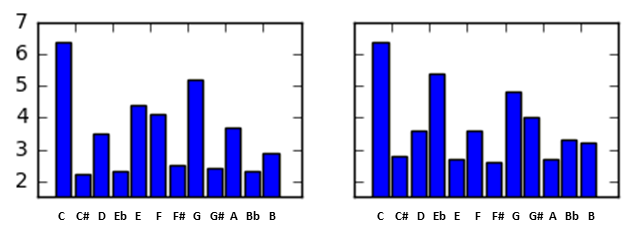
\includegraphics[width=3.1in,angle=0]{imgs/Krumhansl.png}
\caption{Tone profiles derived from the experience conducted by Krumhansl, and representing the C major and the C minor scales, respectively.}
\label{krumhansl}
\end{center}
\end{figure}

Although these two tone profiles provide satisfactory results when the spectrum is approximated by the Constant-Q transform, they are no longer valid 
when the Lomb-Scargle method is used, since it was observed that periodograms consist of coefficients that are broadly distributed more evenly. This distribution has to be reflected in the tone profiles and that is why the algorithm has been evaluated a sufficient number of times, until the tone profiles
provide satisfying results. The adjusted tone profiles are shown in the figure \ref{profiles}.

\begin{figure}
\begin{center}
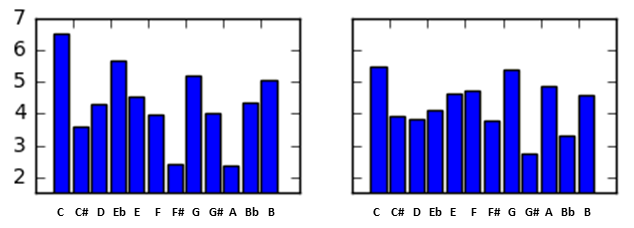
\includegraphics[width=3.1in,angle=0]{imgs/Custom.png}
\caption{Best tone profiles, determined empirically and adjusted for the Lomb-Scargle periodogram}
\label{profiles}
\end{center}
\end{figure}

\subsubsection{Hidden Markov Models (HMM)}
\label{sssec:hmm}

Hidden Markov Models are discrete state machines that represent multivariate series by their distributions and by
the transition probailities between their states. Their states are called “hidden” because they are not observed directly,
but can be inferred from the observation sequence using a parameter estimation method (such as the expectation-maximization algorithm
or the Viterbi algorithm). Each hidden state distinguishes itself by its emission probabilities (or emission probability density function).
Unlike more popular machine learning models such as neural networks or support vector machines (SVM), Hidden Markov Models are capable of
processing input sequences of variable length. This characteristic is substantial given that music tracks are of variable length by nature.\\

The old-fashioned way to classify keys using HMMs consists of training a HMM for each distinct music key, and to predict the most probable 
key of an unlabelled music track by looking for the HMM that maximizes the track\textquotesingle s log-likelihood.

TODO : \citep{JP} \citep{DR}

\subsubsection{Feedforward neural networks}

Neural networks have already delivered good results for classifying chords inside a same piece of music. \citep{JO}

\subsubsection{Input-Output Hidden Markov Models (IO-HMM)}
\label{sssec:iohmm}

The main deficiency of the standard HMM is that it has no discriminative capabilities : if one of the keys appears to be more frequent in the database or
if it seems to be easily explained by the HMM, the latter will present high risks of predicting the same key every time, regardless of the
input sequence. On the other hand, feedforward neural networks have the defect that they are not suited for temporal data, since they must 
process feature vectors of fixed size. [[ TODO : recurrent networks ]]

The Input-Output Hidden Markov Model is well suited for our task because it is affected by none of these deficiencies.

TODO : \citep{YB}

\section{Methodology}


\subsection{Clojure implementation}

Clojure is a dynamic and functional programming language based on the Java Virtual Machine, suited for quickly designing multithreaded programs,
and featuring a full range of immutable and/or persistent data structures. It benefits from both the advantages of compiled languages and dynamic typed
languages, which allows us to write optimized code in a small amount of time, using a fancy syntax. However, although Java libraries can be imported into the Clojure environnement, there is a comparatively small number of libraries that are natively implemented in Clojure. In our case, the majority of the functionalities
are implemented exclusively for the project. Because the Clojure machine learning libraries are at their first steps, we are not using any machine learning 
technique in the design of the final algorithms.\\

The objective of this section is to describe the functional solution design for Clojure, and compare the Lomb-Scargle periodogram and the direct spectral kernel
transform in terms of speed and accuracy. Finally, we will insist on the choices that differ from state of the art from a theoretical point of view.\\

In order to test the numerous features of the project, unit tests have been implemented. In addition, Tufte (a Clojure profiling library) has been used to assess the performance of the various parts of the system. For all the performance-critical areas of the code, we will see the different measures shown by Tufte.\\

\subsection{Solution design}

\begin{figure}[h!]
\begin{center}
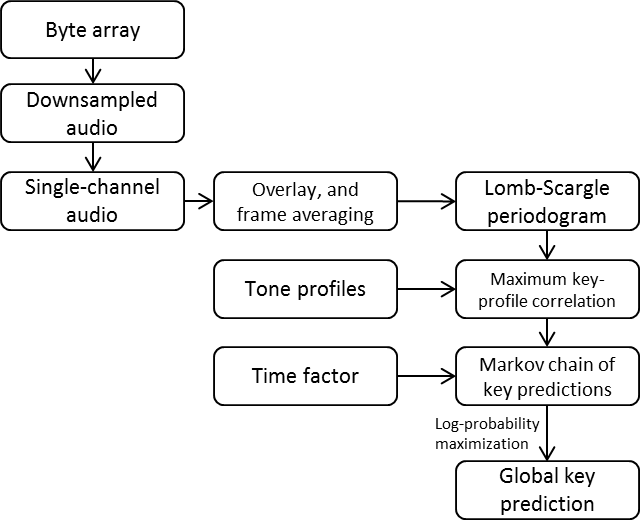
\includegraphics[width=3.1in,angle=0]{imgs/flowChart.png}
\caption{Flowchart : solution design}
\label{fig3}
\end{center}
\end{figure}

\subsubsection{Downsampling and channel averaging}

Since downsampling without filtering has no significative impact on the accuracy, a dedicated wav file reader has been designed to convert a byte stream directly
at the target sampling rate. This is to process far less data samples, thus helping to gain speed. In addition, the downsampled signal is then returned as
a lazy Clojure sequence, ensuring that we don\textquotesingle t evaluate data samples we are not using in the end.
The next step consists of, in the case of a multi-channel audio, averaging the multiple channels. The result of this operation yields a lazy sequence, following
the same logic.

\subsubsection{Lomb-Scargle periodogram}

Considering the spectral estimation remains the performance-critical area of the code, regardless of the technique used, type hints have been added to the functions and var names involved. This is to help the compiler infer the type of return values at compile-time.
At this stage of the code, we are only handling primitives and \textit{clojure.lang.LazySeq} objects (Clojure lazy sequences).\\

We know from equations \ref{fig:cc} and \ref{fig:ss} that the terms CC and SS can be pre-calculated. As a consequence, they are computed at compile-time,
for every trial frequency, and can be reused for each spectral estimation. For this reason, a vector of \textit{PreprocessedWaveforms} objects has been statically defined. A \textit{PreprocessedWaveforms}
type regroups a specific trial frequency, the associated phase change, sine wave and cosine wave, and the corresponding CC and SS terms.\\

\subsubsection{Direct spectral kernel transform}

TODO

\subsubsection{Datasets}

The database consists of 415 music tracks recorded in wav format, 44100 Hz stereo, associated with a labelled key (determined beforehand). 
All keys have been determined
by experts and have been made available by Ibrahim Shat\textquotesingle ath as part of its work. For evaluating algorithms based on MKC,
all the tracks have been used to tune the parameters to their best value. The latter consist of : the major and minor tone profile coefficients,
the size of the sliding window, the frequency range of the spectrum, and the parameter $p$. For evaluating machine learning techniques,
the dataset has been split into a training set of 138 music tracks and a validation set of 277 tracks.

\subsubsection{Evaluation}

In the framework of this study, we consider only the twelve heptatonic major scales and the twelve heptatonic minor scales.
Two different metrics are used to evaluate the accuracy of the algorithms :
the raw accuracy (the ratio between the number of correct predictions to the number of analyzed files) and the MIREX index.
The MIREX metric is a weighted sum of the number of correct predictions (C), the number of predictions that are out by a fifth (F), 
out by a fourth (U), the number of predicted scales that are parallel to the correct ones (P), and the number of predicted scales
that are relative to the correct ones (R). The index is then given by : \\

\noindent $ MIREX = (C + \frac{1}{2}.F + \frac{1}{2}.U + \frac{3}{10}.R + \frac{1}{5}.F) / TOTAL $

\section{Results}

It comes out of this study that the results are much better if we set the parameter $p$ to zero, regardless of the spectral estimation technique used.
The optimal tone profile coefficients are shown in the figure \ref{profiles}. For both DSKT and LS methods, a window size of 4096 samples has provided good results, with an overlap of 4096 samples with the next chunk for the LS periodogram.
Considering a frequency band bounded by $G\#_{-1}$ and $G\#_{5}$ seems to be sufficient to cover the whole spectrum : no significant accuracy improvement has been noticed while increasing the frequency range.

\begin{table}
\center{
\begin{tabular}{|c|c|c|c|}\hline
Method & Accuracy & MIREX & $\tau$ \\ \hline\hline
DSKT (Java FFT) & -  & - & - \\
DSKT (Clojure FFT) & -  & - & - \\
Lomb-Scargle (Clojure) & -  & - & - \\
\hline
\end{tabular}
}
\vskip 0.25cm
\caption{Accuracy assessment, according to the raw accuracy and the MIREX index}
\end{table}

\begin{table}
\center{
\begin{tabular}{|c|c|c|}\hline
Method & Accuracy & MIREX \\ \hline\hline
CQT + MKC & 30,7\%  & - \\
Lomb-Scargle + MKC & 36,6\% & 49,4\% \\
CQT + HMM & -- & -- \\
FFT + IO-HMM & -- & -- \\
CQT + IO-HMM & -- & -- \\ 
Lomb-Scargle + IO-HMM & -- & -- \\ 
\hline
\end{tabular}
}
\vskip 0.25cm
\caption{Accuracy assessment, according to the raw accuracy and the MIREX index}
\end{table}


\begin{table}
\center{
\begin{tabular}{|c|c|c|}\hline
Lomb-Scargle + MKC & Accuracy & MIREX \\ \hline\hline
4096 samples & 30,7\%  & - \\
8192 samples & 37,1\% & 48,9\% \\
12288 samples & 35,9\% & 48,0\% \\
16384 samples & 35,8\% & 48,9\% \\
\hline
\end{tabular}
}
\vskip 0.25cm
\caption{Scores obtained using Lomb-Scargle + MKC, based on the temporal window size}
\end{table}

\footnotesize
\bibliographystyle{apalike}
\bibliography{thesis}

\newpage

\section{Appendices}

\subsection{Appendix A - IOHMM parameters}

\begin{table}
\center{
\begin{tabular}{|c|c|}\hline
Parameter & Value \\ \hline\hline
Topology & linear \\
Number of hidden states & 5 \\
Number of iterations & 25 \\
\hline
\end{tabular}
}
\vskip 0.25cm
\caption{Common parameters of the IO-HMM}
\end{table}

\begin{table}
\center{
\begin{tabular}{|c|c|c|c|}\hline
Parameter & I & S & O \\ \hline\hline
Number of hidden neurons & 20 & 20 & 30\\
Epochs / iteration & 1 & 1 & 1 \\
Hidden activation function & sigmoid & tanh & tanh \\
Learning rate & 0,03 & 0,03 & 0,03 \\
\hline
\end{tabular}
}
\vskip 0.25cm
\caption{Parameters by sub-network type, where $I$ stands for the initial state subnetwork,
$S$ for the state transition sub-networks, and $O$ for the output sub-networks}
\end{table}

\subsection{Appendix B - plots}

\begin{figure}[h!]
\begin{center}
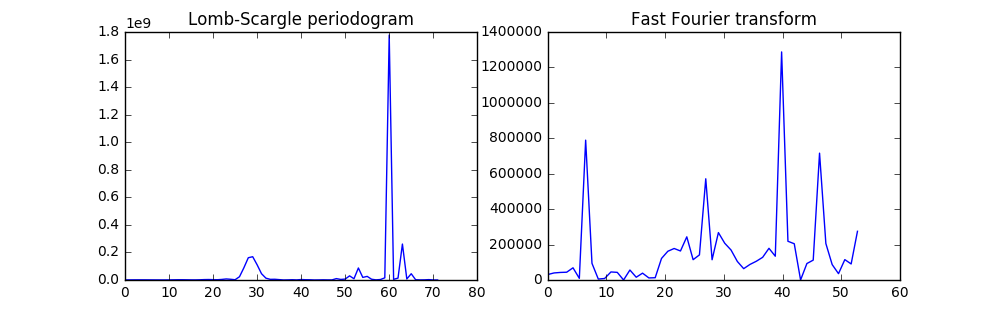
\includegraphics[width=3.1in,angle=0]{imgs/1frame.png}
\caption{Dreadlock holiday - 10cc, frame located at 2 min 44,17 s}
\label{}
\end{center}
\end{figure}

\begin{figure}[h!]
\begin{center}
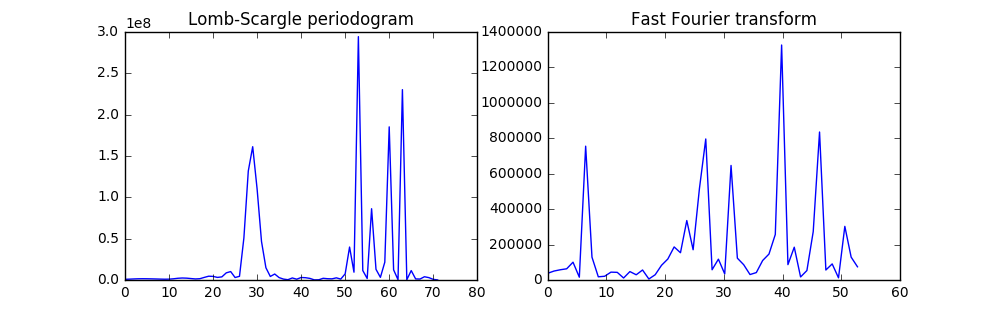
\includegraphics[width=3.1in,angle=0]{imgs/2frames.png}
\caption{Dreadlock holiday - 10cc, frames located at 2 min 44,17 s and 2 min 44,27 s}
\label{}
\end{center}
\end{figure}

\end{document}